%% beamerthemeImperialPoster v1.0 2016/10/01
%% Beamer poster theme created for Imperial College by LianTze Lim (Overleaf)
%% LICENSE: LPPL 1.3
%%
%% This is the example poster demonstrating use
%% of the Imperial College Beamer Poster Theme
\documentclass[xcolor={table}]{beamer}
%% Possible paper sizes: a0, a0b, a1, a2, a3, a4 (although Imperial College posters are usually A0 or A1).
%% Possible orientations: portrait, landscape
%% Font sizes can be changed using the scale option.
\usepackage[size=a0,orientation=portrait,scale=1.55]{beamerposter}
\usepackage{wrapfig}
\usepackage{graphicx}
\usepackage[caption=false,font=footnotesize]{subfig}

\usetheme{ImperialPoster}

%% Four available colour themes
\usecolortheme{ImperialWhite} % Default
% \usecolortheme{ImperialLightBlue}
% \usecolortheme{ImperialDarkBlue}
% \usecolortheme{ImperialBlack}

\title{Disobedience as a Mechanism of Change}


\author{David Burth Kurka\Tsup{1}, Jeremy Pitt\Tsup{1},
 Peter Lewis\Tsup{2}, Alina Patelli\Tsup{2} and Anikó Ekárt\Tsup{2}}

\institute{\Tsup{1}Department of Electrical and Electronic Engineering, Imperial College London\\
\Tsup{2}Aston Lab for Intelligent Collectives Engineering, Aston University}

% \addbibresource{sample.bib}


\begin{document}
\begin{frame}[fragile=singleslide,t]\centering

\maketitle

\begin{columns}[T]

%%%% First Column
\begin{column}{.42\textwidth}

\begin{block}{Disobedience in Society}

\begin{itemize}

% Iron law of oligarchy
% Principled violation of policy
% Adaptive learning. Learning, adaptation

% Norm-governed multi agent systems
% selective non-application of a sanction.


% Here, we aim to capitalise on all three re-
% search threads presented above, namely, disobedi-
% ence (principled violation of policy), opinion for-
% mation as a safeguard against oligarchy and using
% learning for preserving institutional endurance.

\item \textbf{Disobedience} has been used historically as a form of resistance and call for change in unfair regimes.
\item Among the factors that motivate widespread disobedience are:
\begin{itemize}
    \item \textbf{The iron law of oligarchy} -- The tendency of rulers to change norms to their own benefit.
    \item \textbf{Principled violation of policy} -- Selective common-sense non-application of a sanction.
\end{itemize}
\end{itemize}

\end{block}


\begin{block}{Disobedience as learning mechanism}
\begin{itemize}
\item Can these notions be applied to \textbf{norm-governed MAS}?
\item Can disobedience be a form of \textbf{social learning}, enabling the construction of adaptive systems?
\item How can those concepts enable \textbf{rule- or ruler-change} of corruptive systems?
%
\end{itemize}

\end{block}




\begin{block}{Base premises and operationalisation}

\begin{figure}
  \centering
  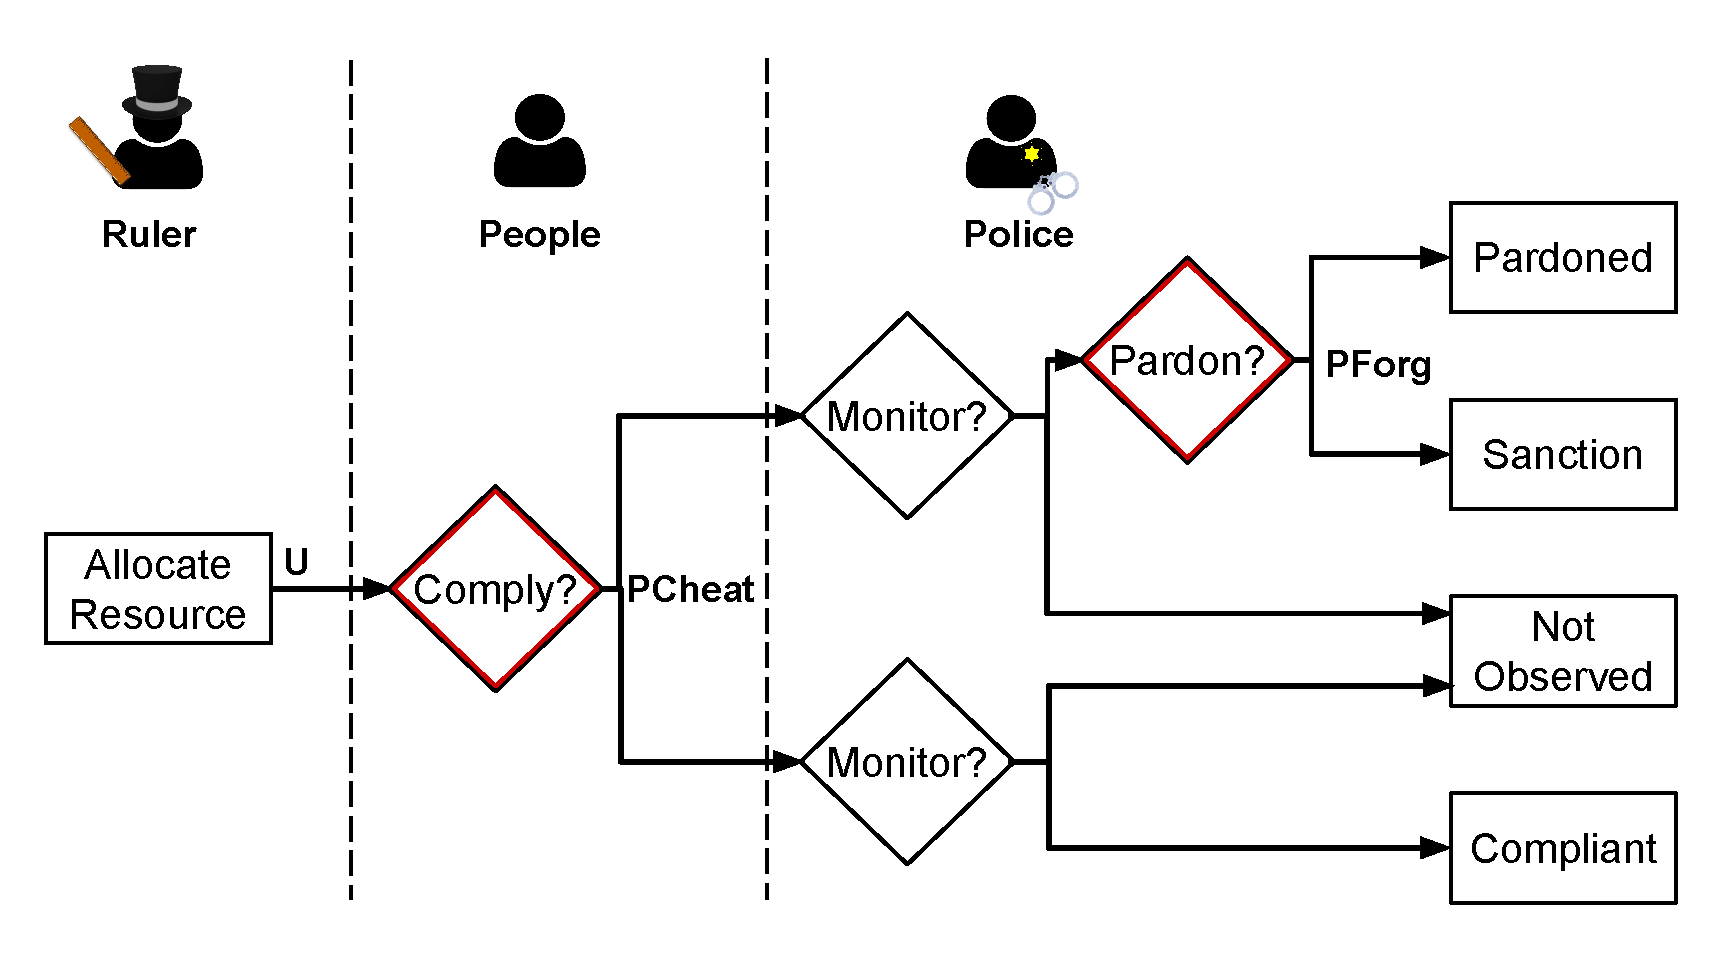
\includegraphics[width=0.9\linewidth]{img/disobedience_flow.pdf}
\end{figure}

\begin{figure}
  \centering
  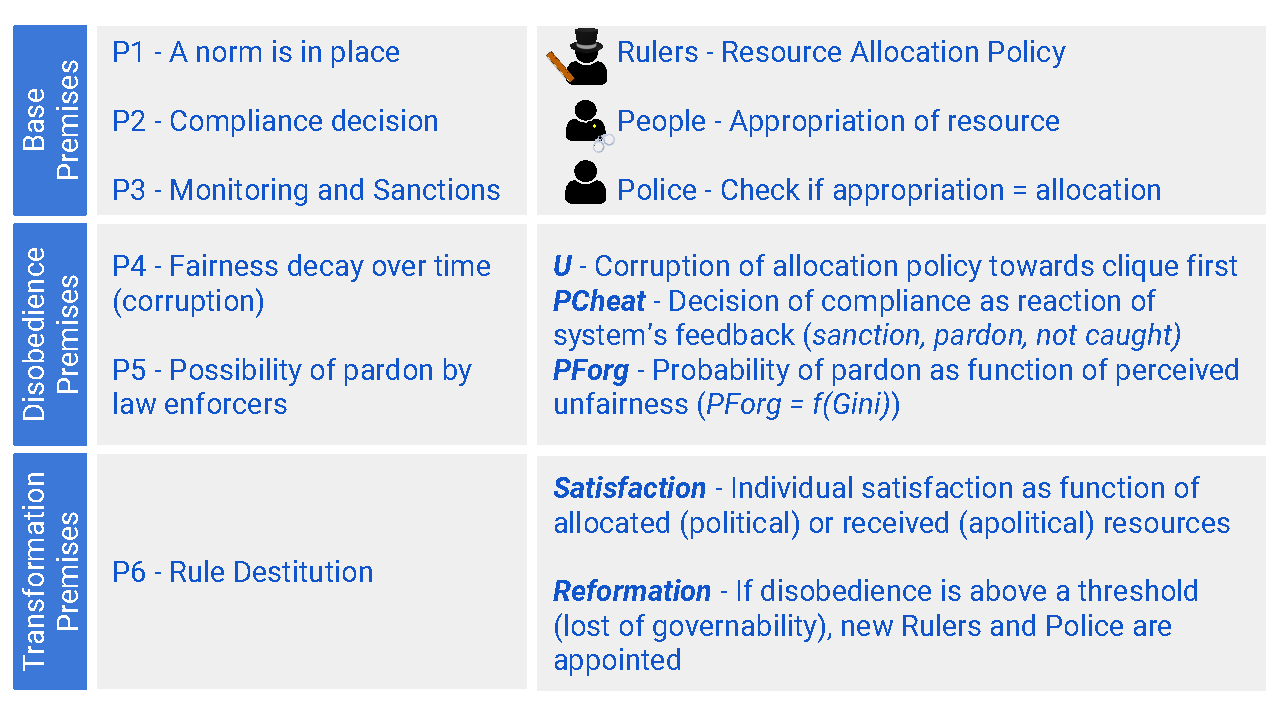
\includegraphics[width=0.9\linewidth]{img/disobedience_summary.pdf}
\end{figure}



\end{block} 

\begin{block}{Exploratory space}
\begin{figure}
  \centering
  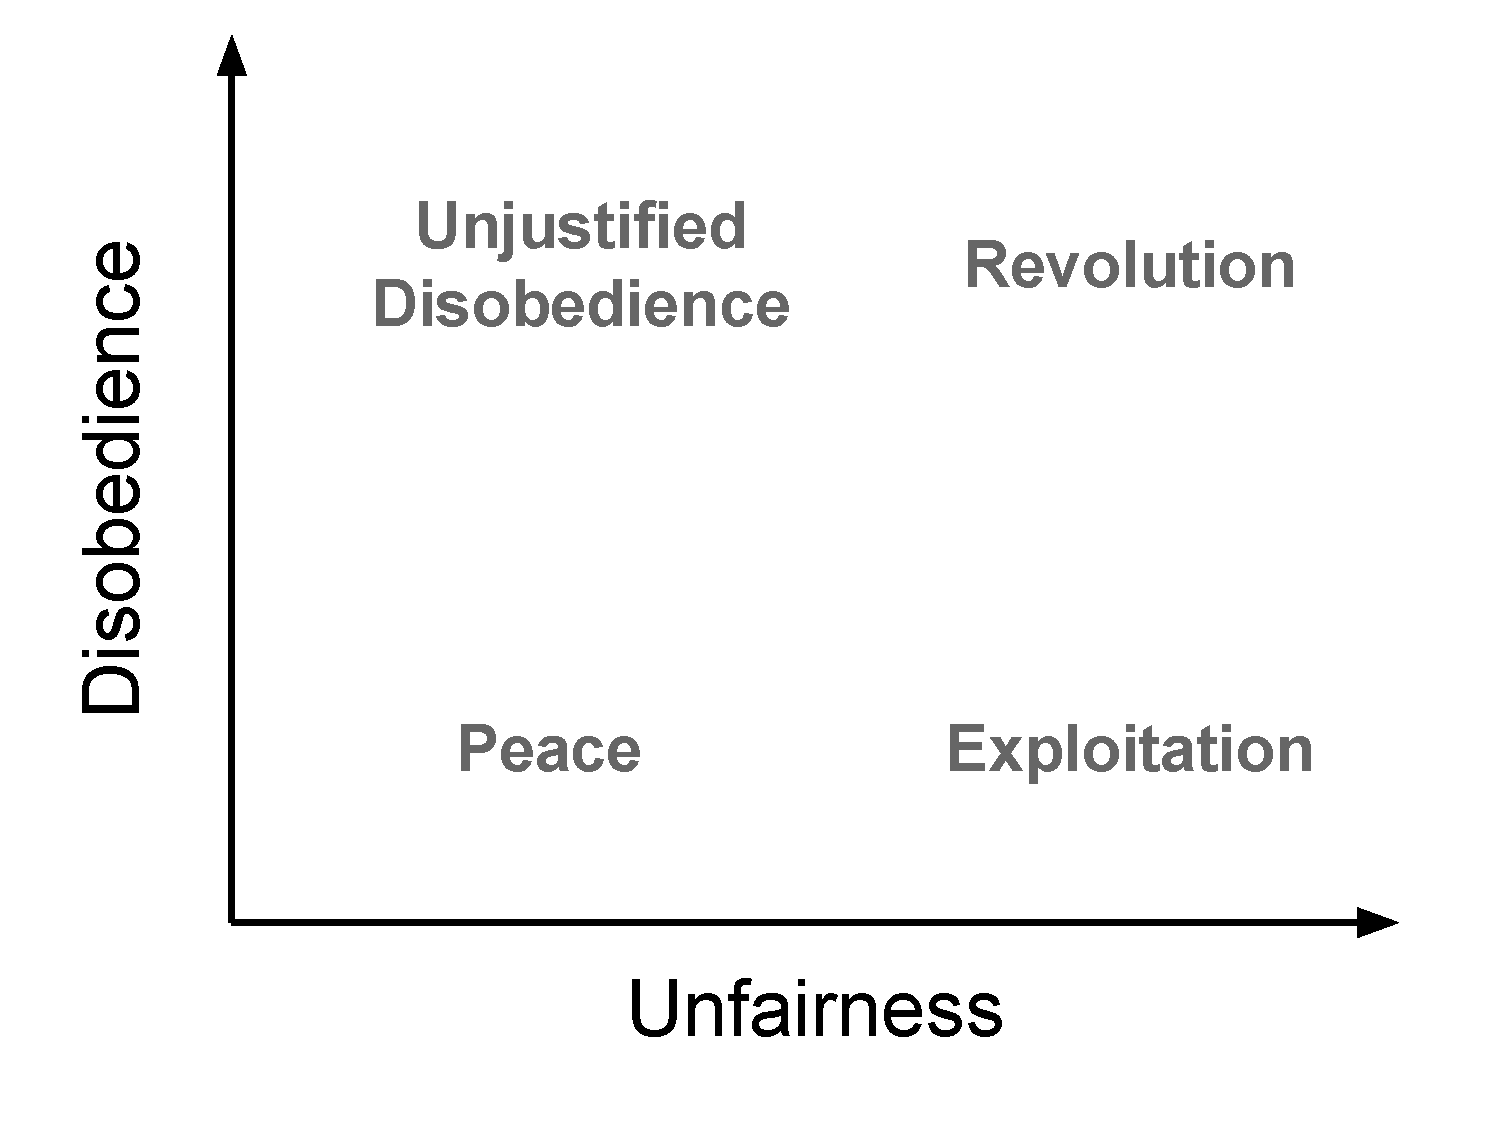
\includegraphics[width=0.8\linewidth]{img/space_disob.pdf} 
\end{figure}
\end{block} 

\end{column}
%%%% Second Column
\begin{column}{.58\textwidth}


\begin{block}{Base Game}

Without pardoning or reformation, People stay at the mercy of rulers, not having another rational choice than obeying, no matter how unfair is the current policy.


\begin{figure}
  \centering
  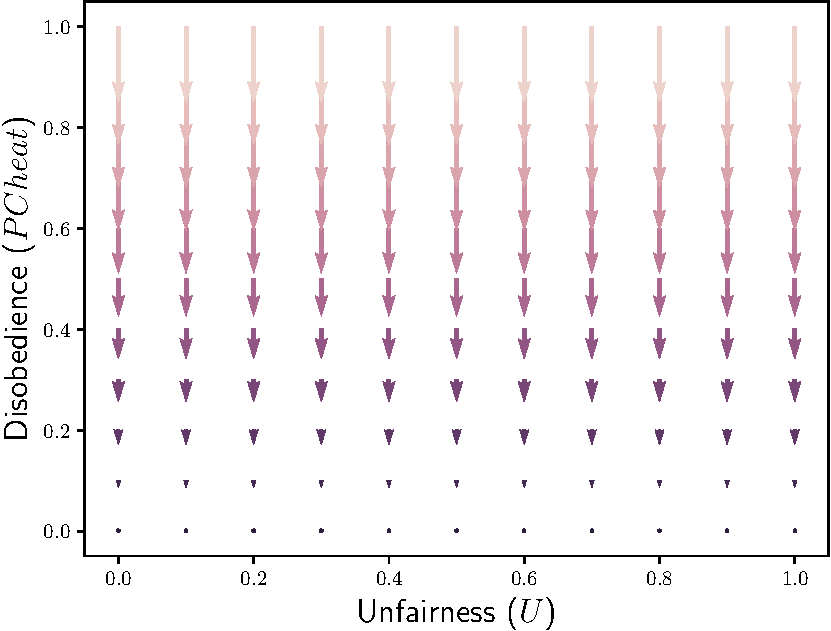
\includegraphics[width=0.55\linewidth]{img/phasebase-crop.pdf} 
\end{figure}


\begin{figure}[H]
  \centering
  \subfloat[Peace]{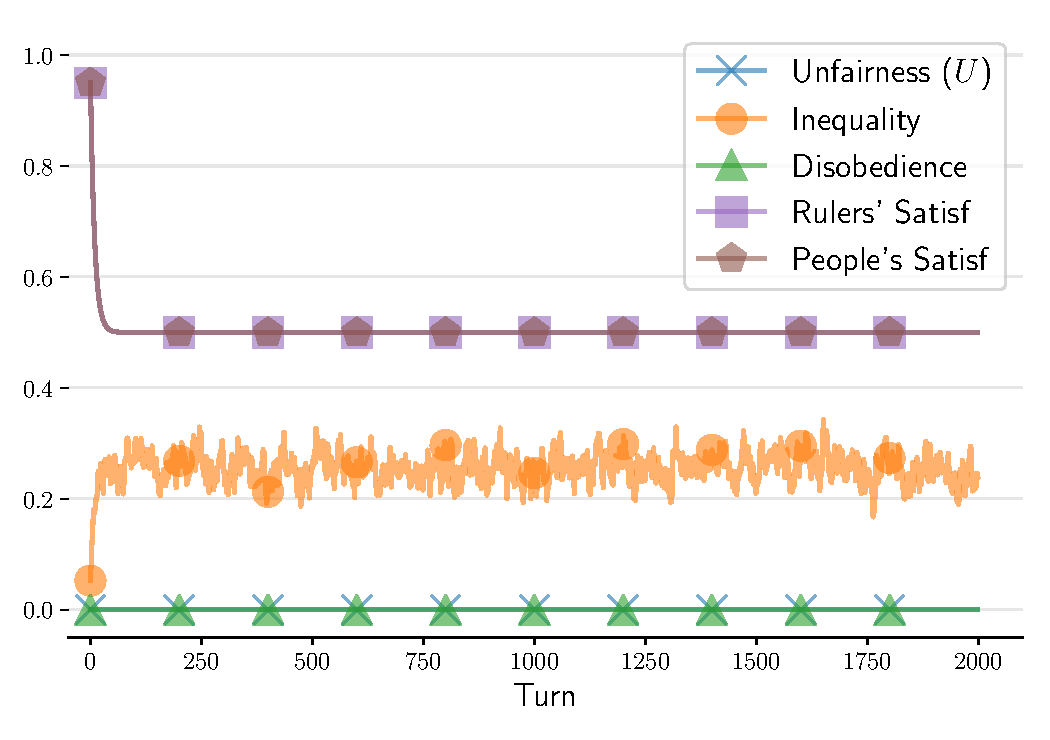
\includegraphics[width=.25\linewidth]{img/timebase.pdf}\label{fig:stability}}
  \subfloat[Unjust.\ Disobedience]{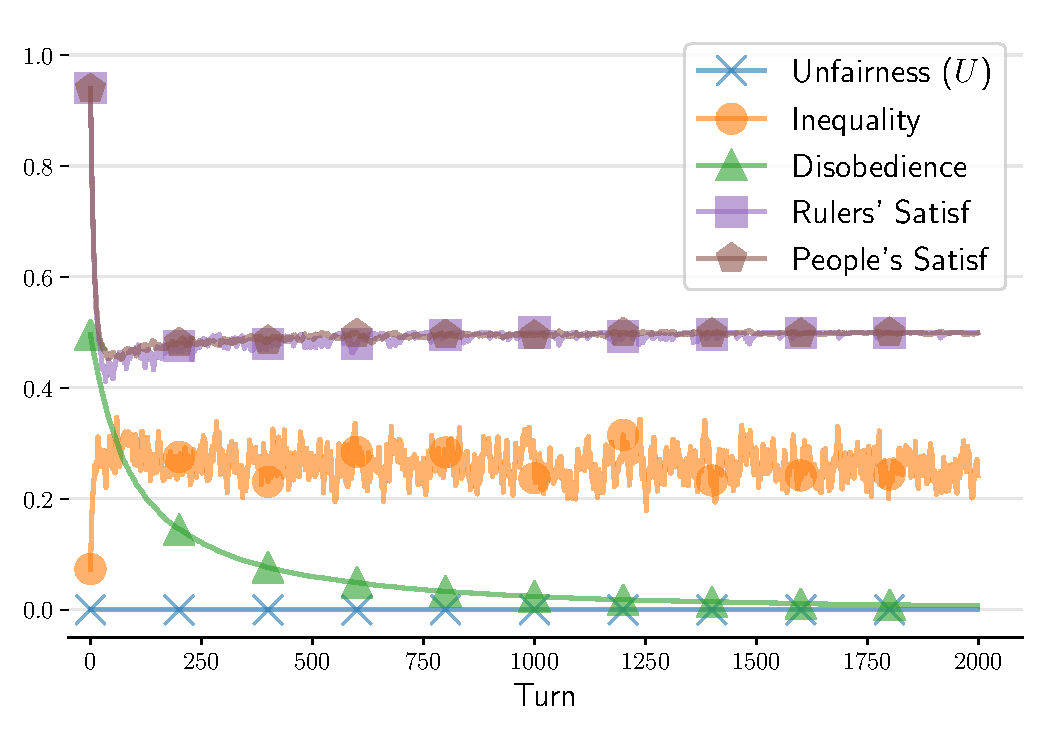
\includegraphics[width=.25\linewidth]{img/timeunjustified.pdf}\label{fig:unjustified}}
  \subfloat[Exploitation]{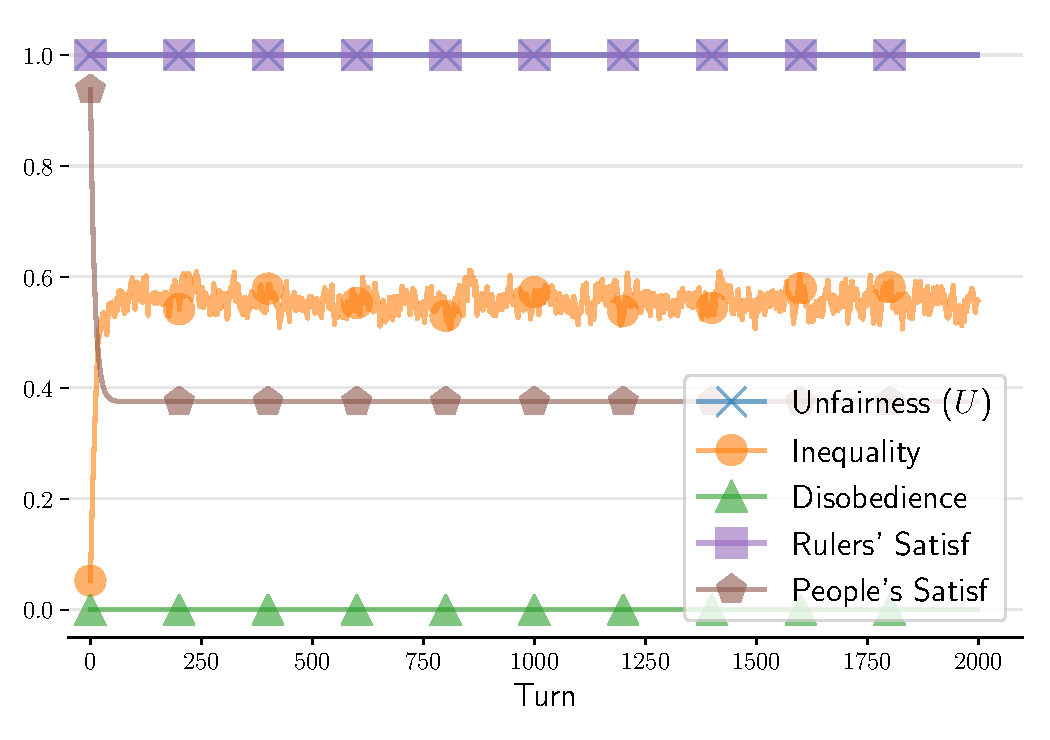
\includegraphics[width=.25\linewidth]{img/timeexploitation.pdf}\label{fig:exploitation}}
\subfloat[Oppression]{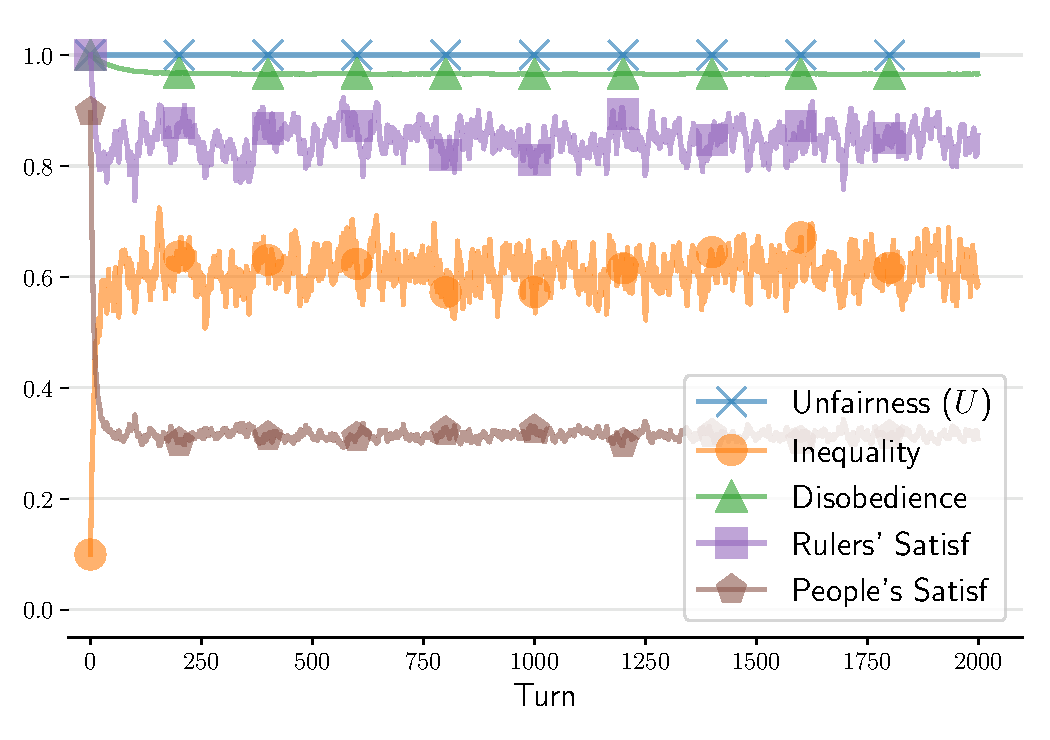
\includegraphics[width=.25\linewidth]{img/timeoppresion.pdf}\label{fig:oppression}}
\end{figure}



\end{block} 



\begin{block}{First Extension -- Pardoning}

Obedience is now conditioned to unfairness level: if fair, agents obey; if unfair, agents tend to non-compliance. Given unfair allocation policy, Police validate norms disobedience, pardoning transgressions. 
% \vspace{20pt}

\begin{columns}[c]
\begin{column}{.6\textwidth}
 
\begin{figure}
  \centering
  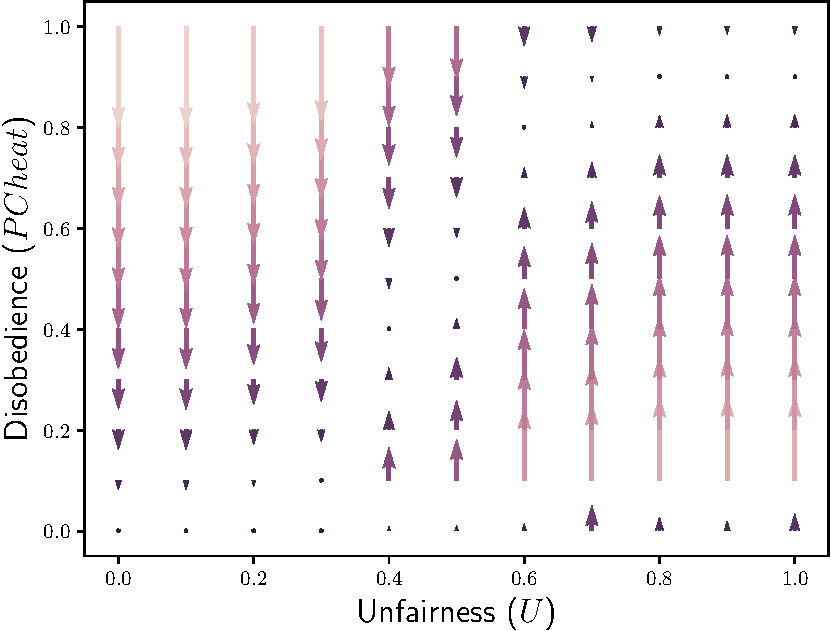
\includegraphics[width=1.0\linewidth]{img/phaseext1.pdf}
%  \caption{Phase plane for Extension 1 (premises 1--5). Obedience is conditioned
%     to unfairness level: if fair, agents obey; if unfair, agents tend to
%     non-compliance.}\label{fig:ext1phase}
\end{figure}

\end{column}
\begin{column}{.4\textwidth}



% \begin{figure}
%   \centering
  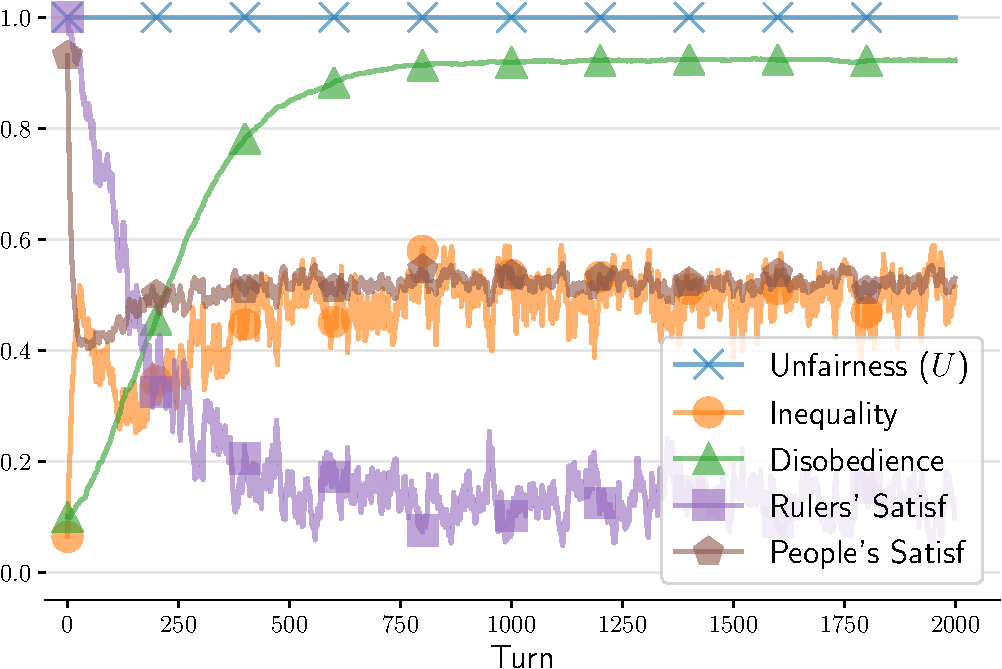
\includegraphics[width=0.9\linewidth]{img/timerevolution.pdf}
% %   \caption{Revolution -- unfair allocation, non-compliance. Given unfair
% % allocation policy, Police validate norms disobedience, pardoning transgressions.
% % Thus agents have space to protest by freely demonstrating their dissatisfaction
% % and appropriating resources, restoring the environment's
% % fairness.}\label{fig:revrulersrandom}
% \end{figure}

Agents can protest by freely demonstrating their dissatisfaction and appropriating resources, restoring the environment's fairness.
\end{column}
\end{columns}





\end{block} 


\begin{block}{Second Extension -- Reformation}
Three possible dynamic equilibria:



\begin{columns}[T]
\begin{column}{.333\textwidth}



\begin{center}
Revolution cycles

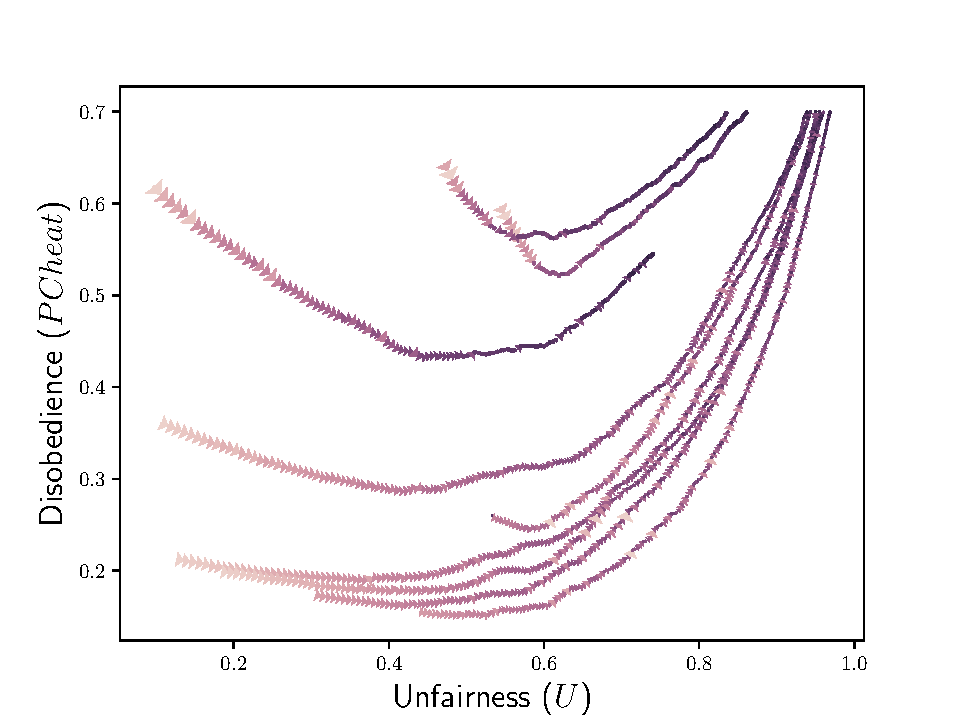
\includegraphics[width=\linewidth]{img/trajext2corrupted.pdf}\label{fig:ext2phase}

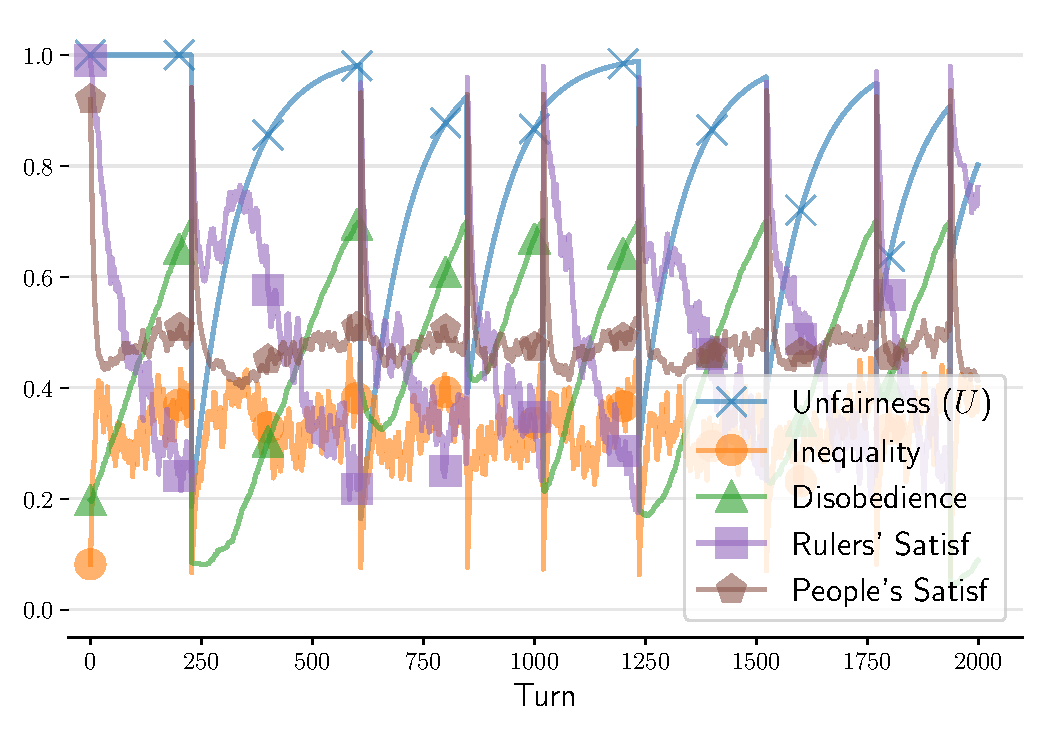
\includegraphics[width=.9\linewidth]{img/timecycle.pdf}\label{fig:revcycle}
\end{center}

\end{column}
\begin{column}{.333\textwidth}



\begin{center}
Popular Control

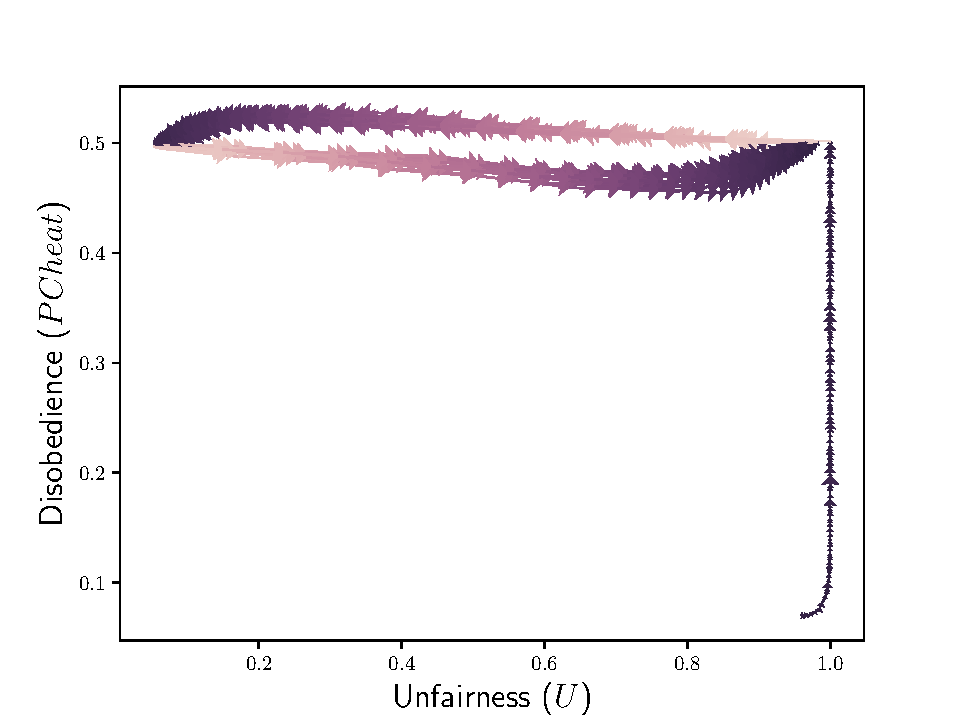
\includegraphics[width=\linewidth]{img/trajtories.pdf}\label{fig:toriesphase}

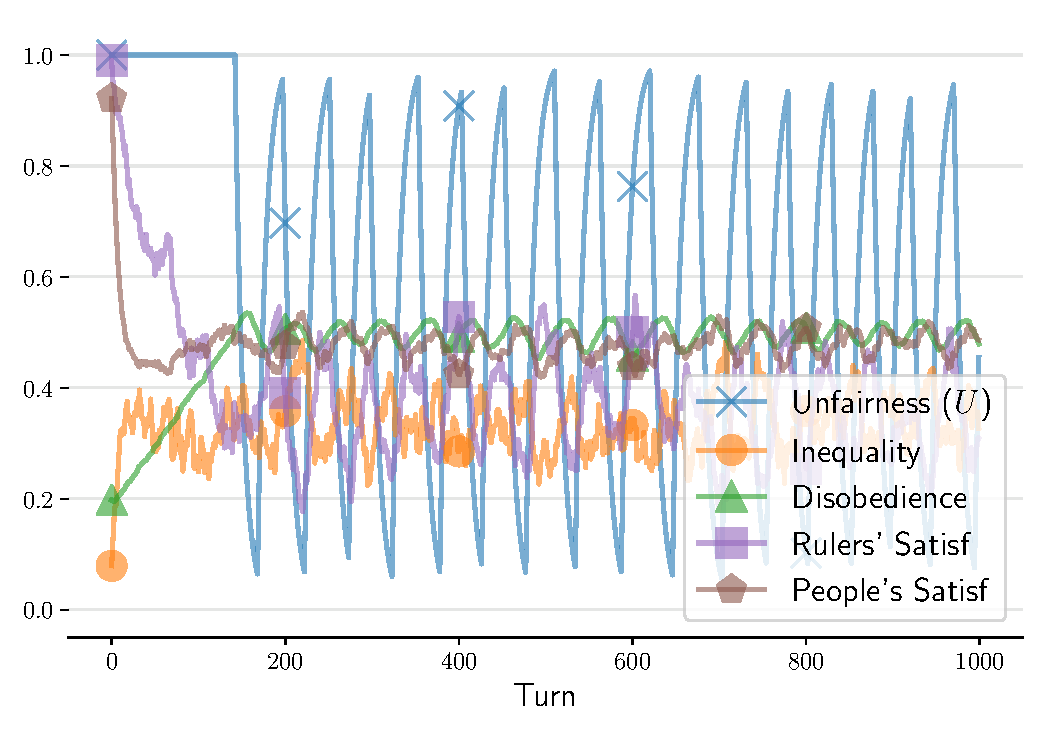
\includegraphics[width=.9\linewidth]{img/timetories.pdf}\label{fig:toriestime}
\end{center}


\end{column}

\begin{column}{.333\textwidth}

\begin{center}
Pragmatic Revolution

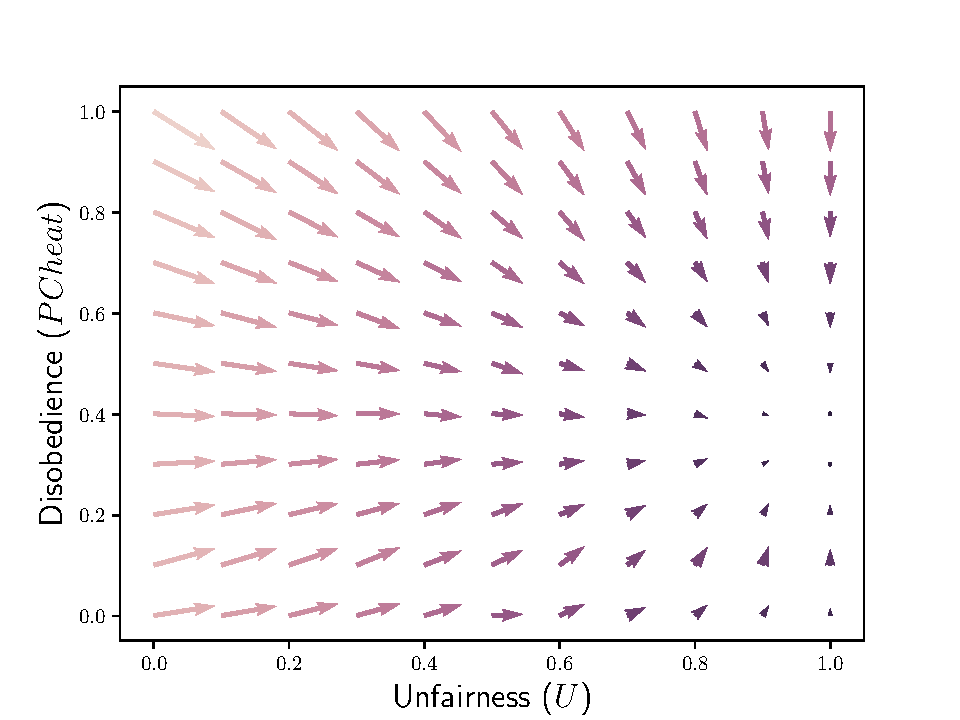
\includegraphics[width=\linewidth]{img/phaseapolitical}

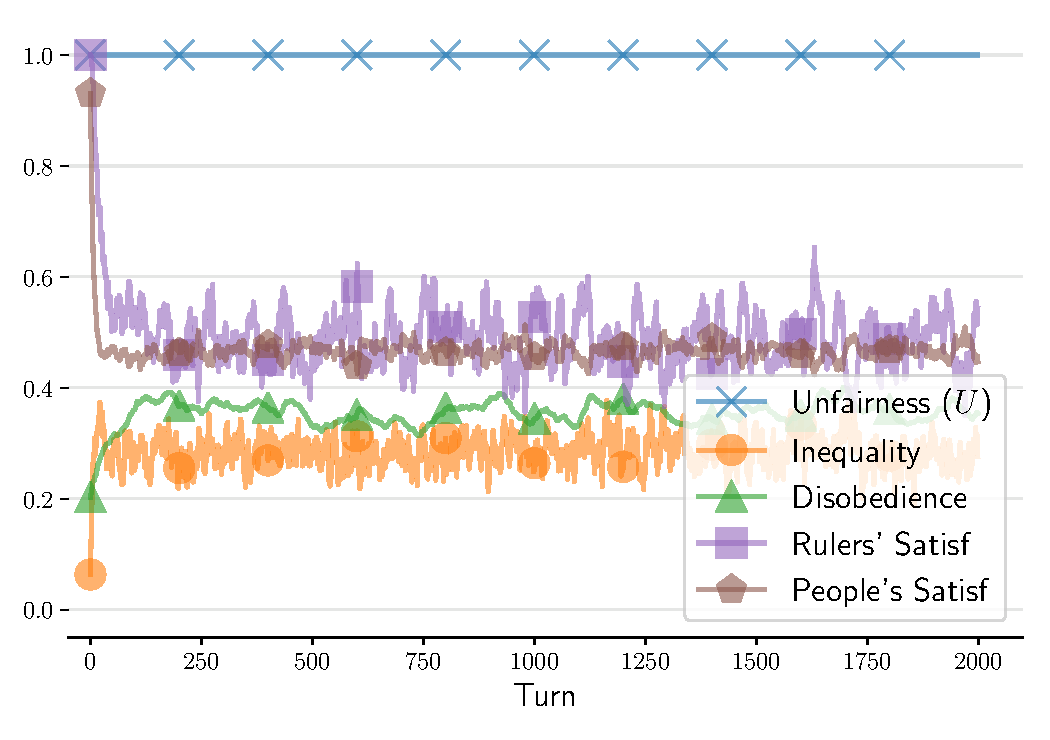
\includegraphics[width=.9\linewidth]{img/timeapolitical.pdf}
\end{center}

\end{column}
\end{columns}

\end{block} 



\end{column}
\end{columns}


\end{frame}
\end{document}
%%% Local Variables:
%%% mode: latex
%%% TeX-master: t
%%% End:
